\newpage

\section{Log of \ref{sec:WBSTaskRepresentation} triple}

%\paragraph Task atomico, non suddiviso in sottotask.
%\begin{sidewaysfigure}[h!] 
%\centering
%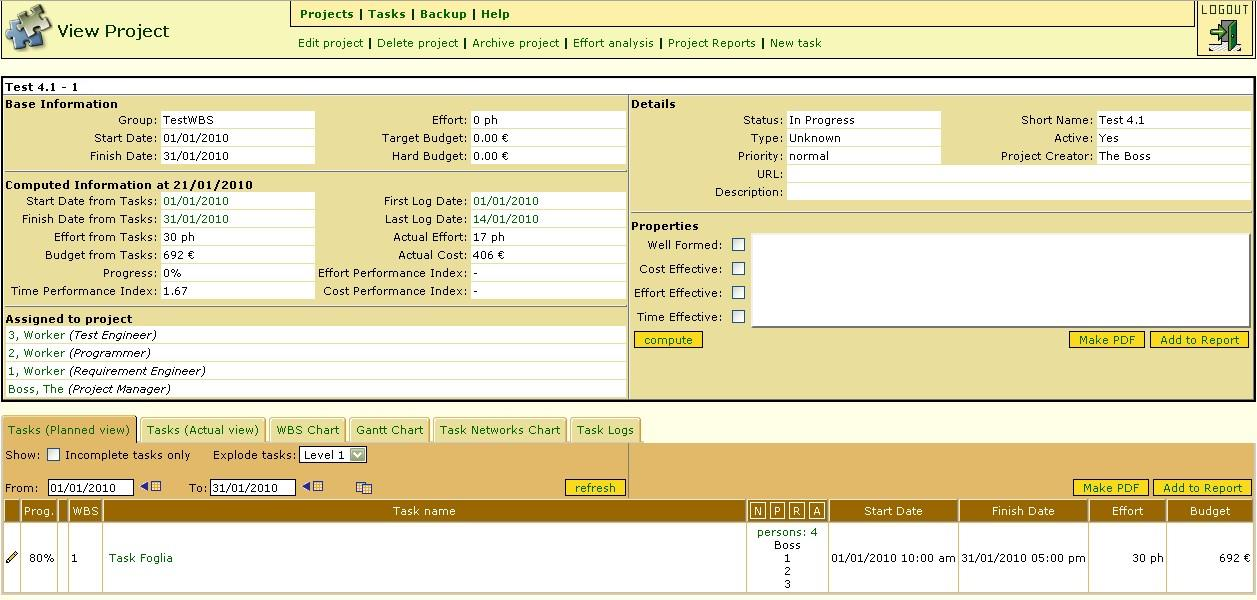
\includegraphics[width=1\textwidth]{tests/TEST_WBS/4.1/4.1_1/Esempio_1/input.png}
%\caption{Input: Planned View}
%\end{sidewaysfigure}
%\newpage


\subsection{Task atomico, non suddiviso in sottotask}
\paragraph{Esempio 1}
\paragraph{Input: Planned view, Actual view}
\begin{figure}[h!]
\centering
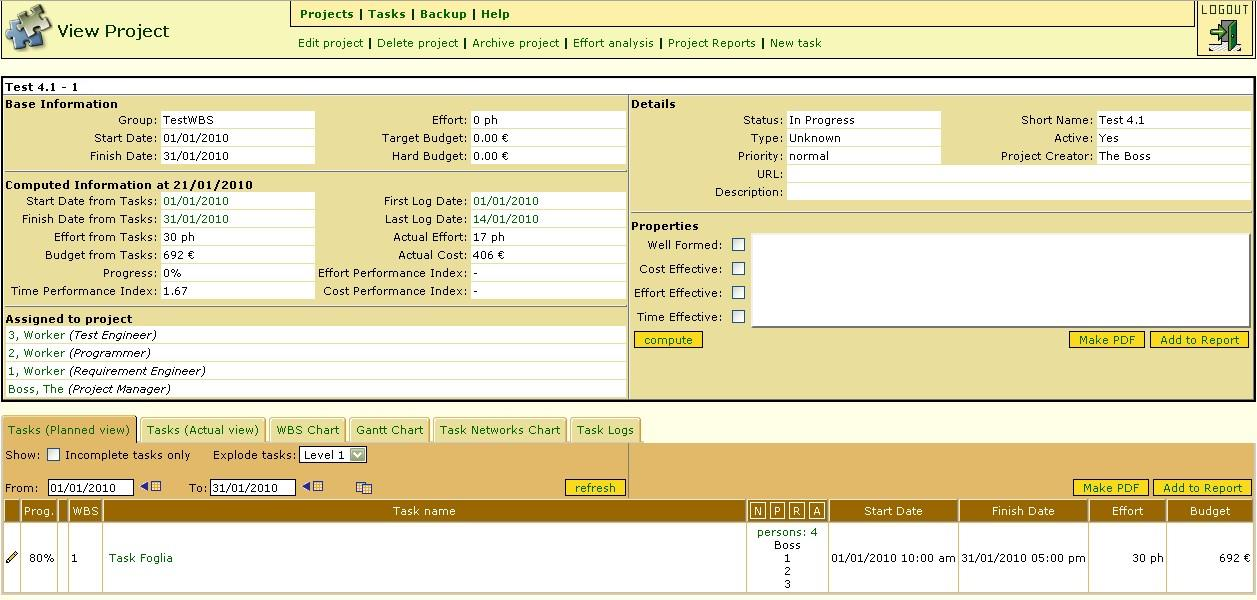
\includegraphics[width=\textwidth]{tests/TEST_WBS/4.1/4.1_1/Esempio_1/input.png}
\end{figure}
\begin{figure}[h!]
\centering
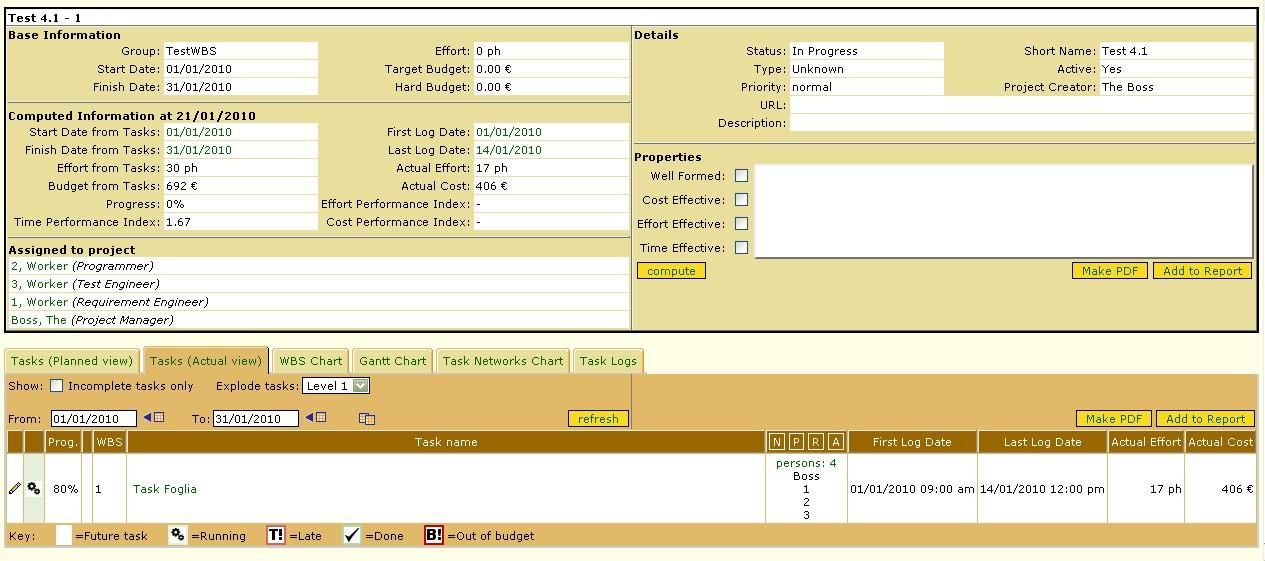
\includegraphics[width=\textwidth]{tests/TEST_WBS/4.1/4.1_1/Esempio_1/input_actual.png}
\end{figure}
\newpage

\paragraph{Environment}
\begin{figure}[h!]
\centering
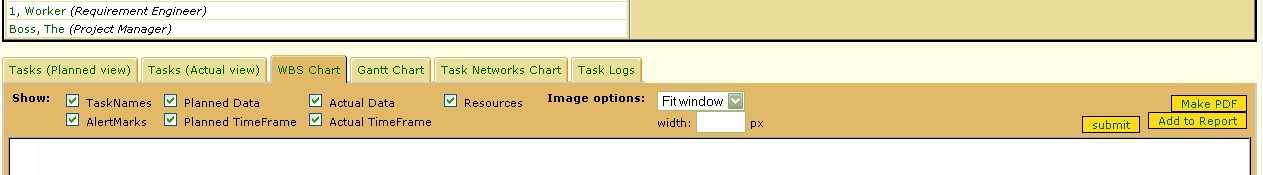
\includegraphics[width=\textwidth]{tests/TEST_WBS/4.1/4.1_1/Esempio_1/environment.png}
\end{figure}

\paragraph{Esito}
\begin{figure}[h!]
\centering

\includegraphics[width=\textwidth]{tests/TEST_WBS/4.1/4.1_1/Esempio_1/output.png}
\end{figure}
\newpage


\paragraph{Esempio 2}
\paragraph{Input: Planned view, Actual view}
\begin{figure}[h!]
\centering
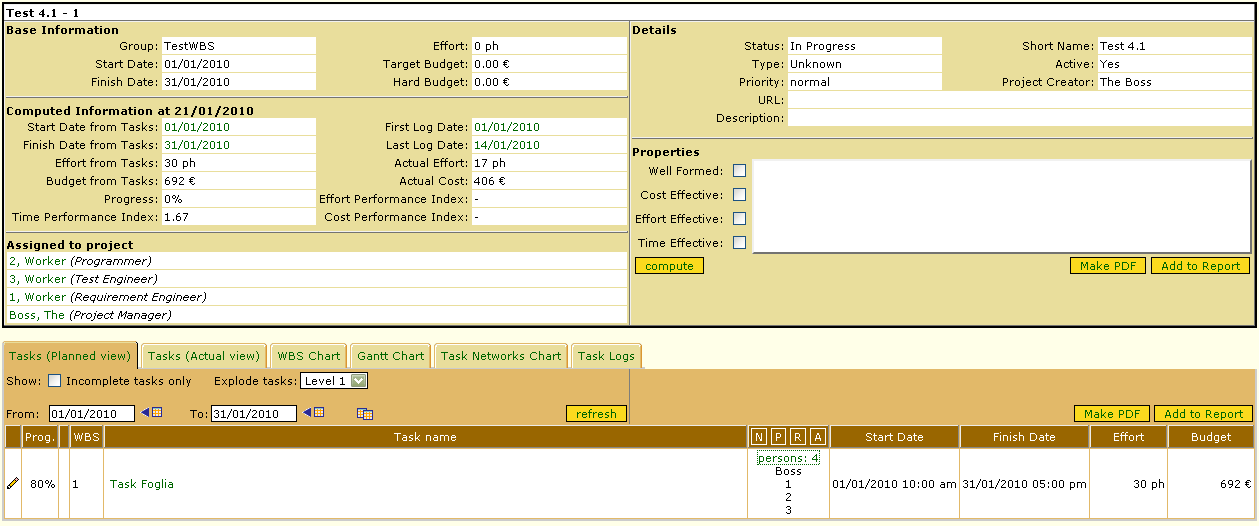
\includegraphics[width=\textwidth]{tests/TEST_WBS/4.1/4.1_1/Esempio_2/input.png}
\end{figure}
\begin{figure}[h!]
\centering
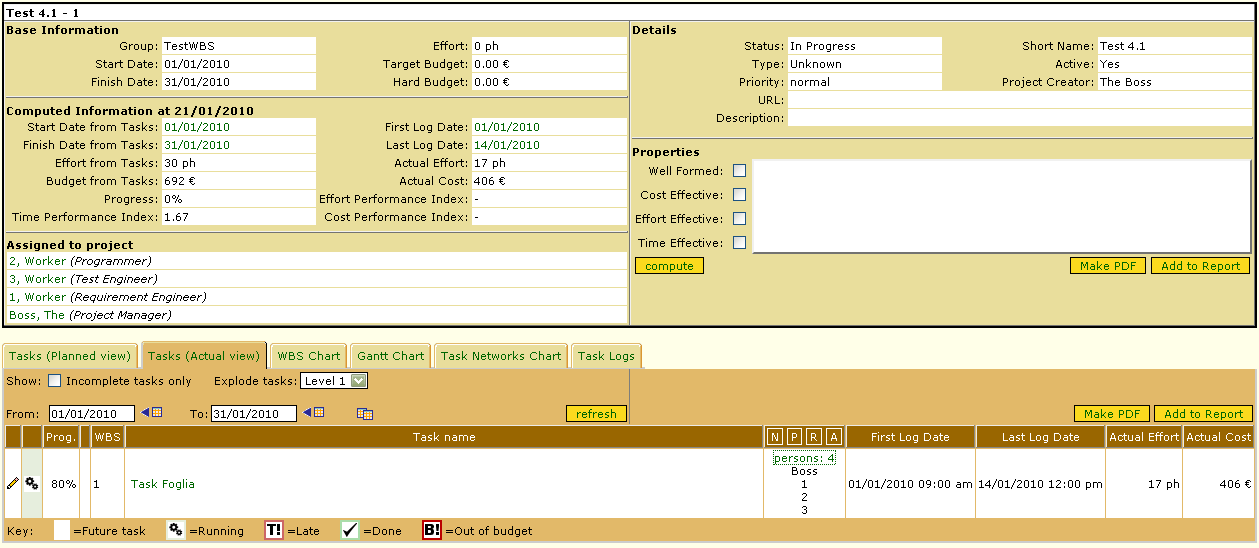
\includegraphics[width=\textwidth]{tests/TEST_WBS/4.1/4.1_1/Esempio_2/input_actual.png}
\end{figure}
\newpage

\paragraph{Environment}
\begin{figure}[h!]
\centering
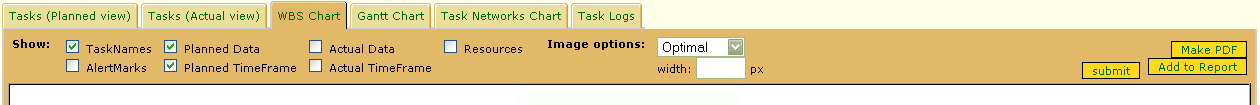
\includegraphics[width=\textwidth]{tests/TEST_WBS/4.1/4.1_1/Esempio_2/environment.png}
\end{figure}

\paragraph{Esito}
\begin{figure}[h!]
\centering

\includegraphics[width=\textwidth]{tests/TEST_WBS/4.1/4.1_1/Esempio_2/output.png}
\end{figure}
\newpage



\paragraph{Esempio 3}
\paragraph{Input: Planned view, Actual view}
\begin{figure}[h!]
\centering
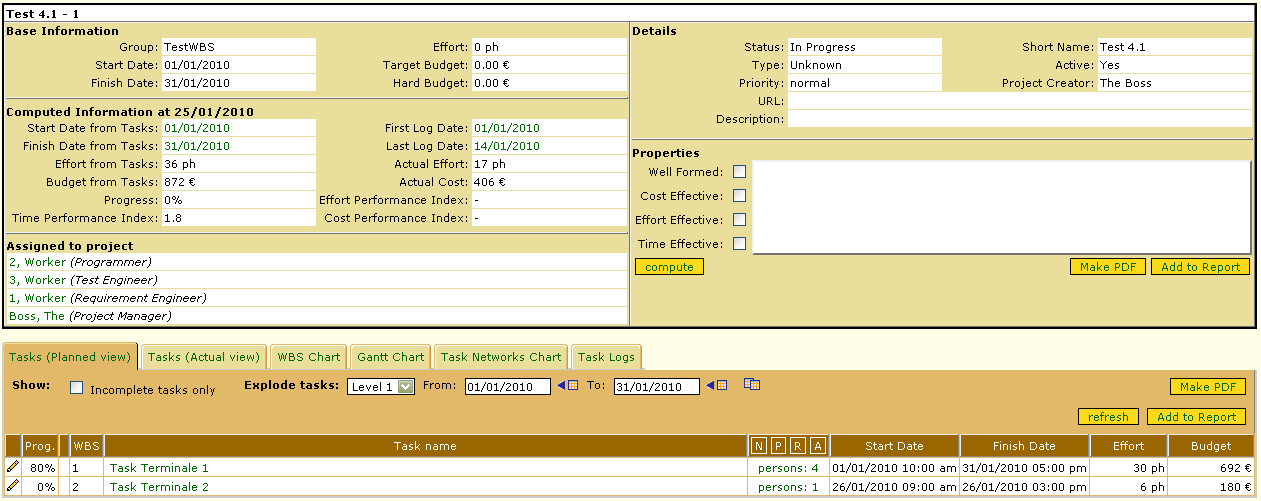
\includegraphics[width=\textwidth]{tests/TEST_WBS/4.1/4.1_1/Esempio_3/input.png}
\end{figure}
\begin{figure}[h!]
\centering
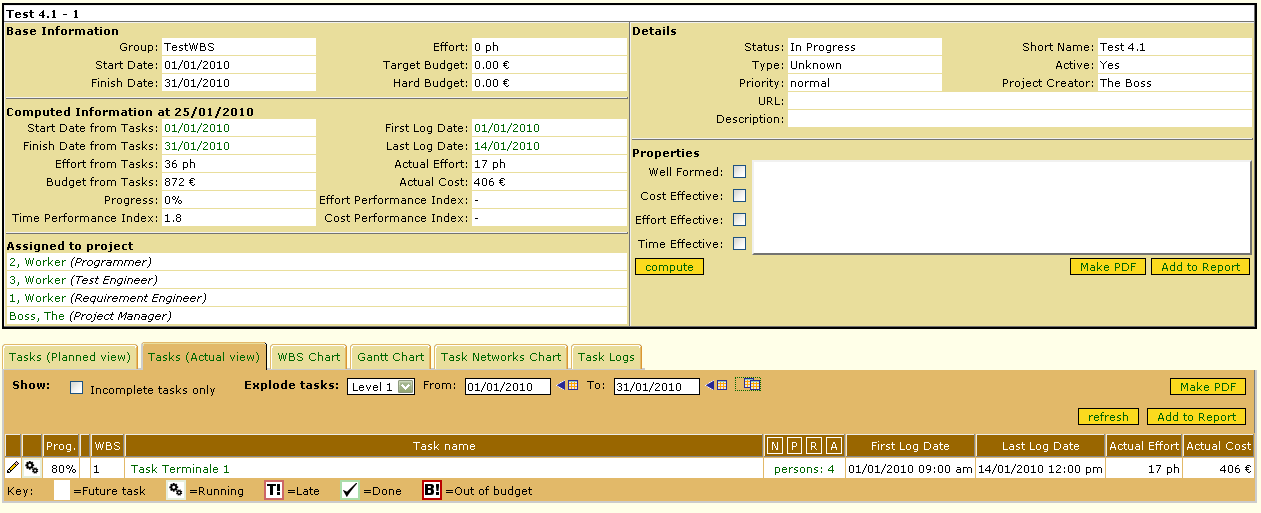
\includegraphics[width=\textwidth]{tests/TEST_WBS/4.1/4.1_1/Esempio_3/input_actual.png}
\end{figure}
\newpage

\paragraph{Environment}
\begin{figure}[h!]
\centering
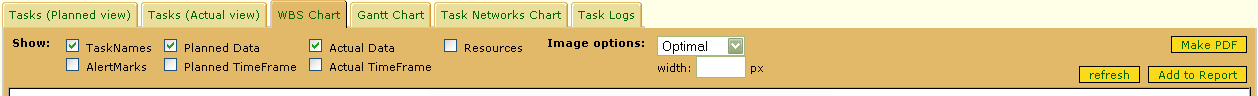
\includegraphics[width=\textwidth]{tests/TEST_WBS/4.1/4.1_1/Esempio_3/environment.png}
\end{figure}

\paragraph{Esito}
\begin{figure}[h!]
\centering

\includegraphics[width=\textwidth]{tests/TEST_WBS/4.1/4.1_1/Esempio_3/output.png}
\end{figure}
\newpage


\subsection{Task composto, visualizzando i sotto task del livello successivo}
\paragraph{Esempio 1}
\paragraph{Input: Planned view, Actual view}
\begin{figure}[h!]
\centering
\includegraphics[width=\textwidth]{tests/TEST_WBS/4.1/4.1_2/Esempio_1/input.png}
\end{figure}
\begin{figure}[h!]
\centering
\includegraphics[width=\textwidth]{tests/TEST_WBS/4.1/4.1_2/Esempio_1/input_actual.png}
\end{figure}
\newpage

\paragraph{Environment}
\begin{figure}[h!]
\centering
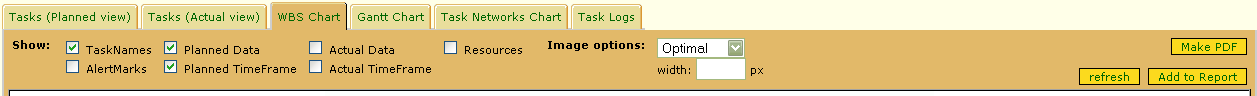
\includegraphics[width=\textwidth]{tests/TEST_WBS/4.1/4.1_2/Esempio_1/environment.png}
\end{figure}

\paragraph{Esito}
\begin{figure}[h!]
\centering

\includegraphics[width=\textwidth]{tests/TEST_WBS/4.1/4.1_2/Esempio_1/output.png}
\end{figure}
\newpage

\paragraph{Esempio 2}
\paragraph{Input: Planned view, Actual view}
\begin{figure}[h!]
\centering
\includegraphics[width=\textwidth]{tests/TEST_WBS/4.1/4.1_2/Esempio_2/input.png}
\end{figure}
\begin{figure}[h!]
\centering
\includegraphics[width=\textwidth]{tests/TEST_WBS/4.1/4.1_2/Esempio_2/input_actual.png}
\end{figure}
\newpage

\paragraph{Environment}
\begin{figure}[h!]
\centering
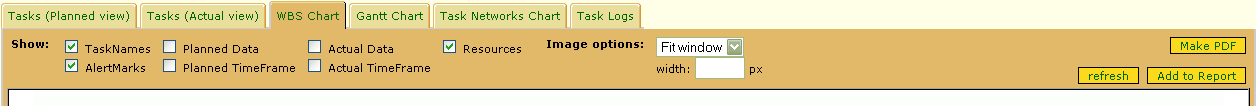
\includegraphics[width=\textwidth]{tests/TEST_WBS/4.1/4.1_2/Esempio_2/environment.png}
\end{figure}

\paragraph{Esito}
\begin{figure}[h!]
\centering

\includegraphics[width=\textwidth]{tests/TEST_WBS/4.1/4.1_2/Esempio_2/output.png}
\end{figure}
\newpage


\subsection{Task composto, collassando i sotto task}
\paragraph{Esempio 1}
\paragraph{Input: Planned view, Actual view}
\begin{figure}[h!]
\centering
\includegraphics[width=\textwidth]{tests/TEST_WBS/4.1/4.1_3/Esempio_1/input.png}
\end{figure}
\begin{figure}[h!]
\centering
\includegraphics[width=\textwidth]{tests/TEST_WBS/4.1/4.1_3/Esempio_1/input_actual.png}
\end{figure}
\newpage

\paragraph{Environment}
\begin{figure}[h!]
\centering
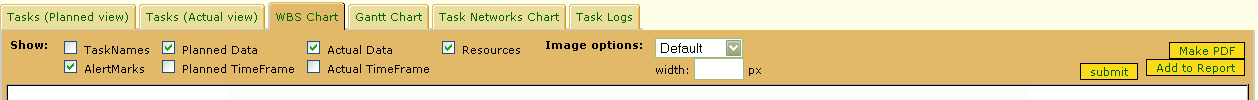
\includegraphics[width=\textwidth]{tests/TEST_WBS/4.1/4.1_3/Esempio_1/environment.png}
\end{figure}

\paragraph{Esito}
\begin{figure}[h!]
\centering

\includegraphics[width=\textwidth]{tests/TEST_WBS/4.1/4.1_3/Esempio_1/output.png}
\end{figure}
\newpage

\paragraph{Esempio 2}
\paragraph{Input: Planned view, Actual view}
\begin{figure}[h!]
\centering
\includegraphics[width=\textwidth]{tests/TEST_WBS/4.1/4.1_3/Esempio_2/input.png}
\end{figure}
\begin{figure}[h!]
\centering
\includegraphics[width=\textwidth]{tests/TEST_WBS/4.1/4.1_3/Esempio_2/input_actual.png}
\end{figure}
\newpage

\paragraph{Environment}
\begin{figure}[h!]
\centering
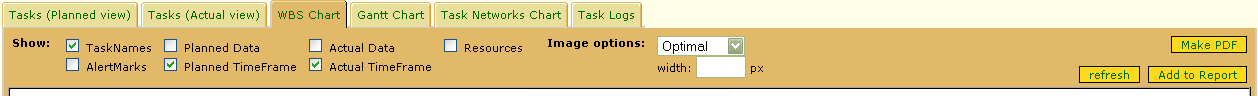
\includegraphics[width=\textwidth]{tests/TEST_WBS/4.1/4.1_3/Esempio_2/environment.png}
\end{figure}

\paragraph{Esito}
\begin{figure}[h!]
\centering

\includegraphics[width=\textwidth]{tests/TEST_WBS/4.1/4.1_3/Esempio_2/output.png}
\end{figure}
\newpage


\subsection{Possibili varianti di task: coerenti, in anticipo, in ritardo, troppo costosi, non ancora loggati}

\paragraph{Esempio 1}
\paragraph{Input: Planned view, Actual view}
\begin{figure}[h!]
\centering
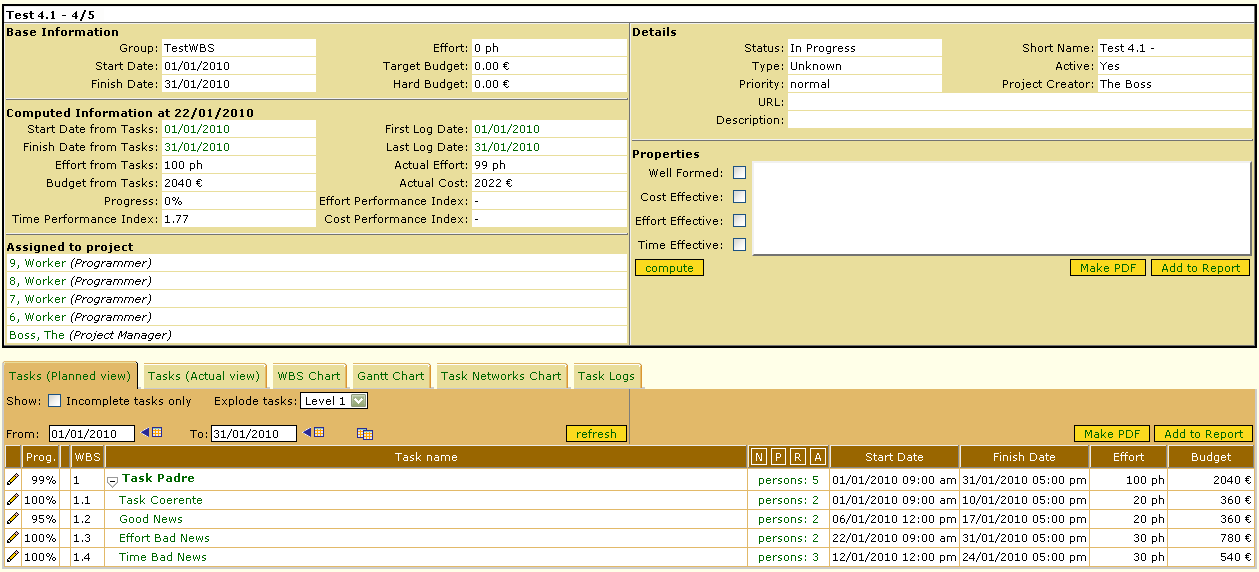
\includegraphics[width=\textwidth]{tests/TEST_WBS/4.1/4.1_4_5/Esempio_1/input.png}
\end{figure}
\begin{figure}[h!]
\centering
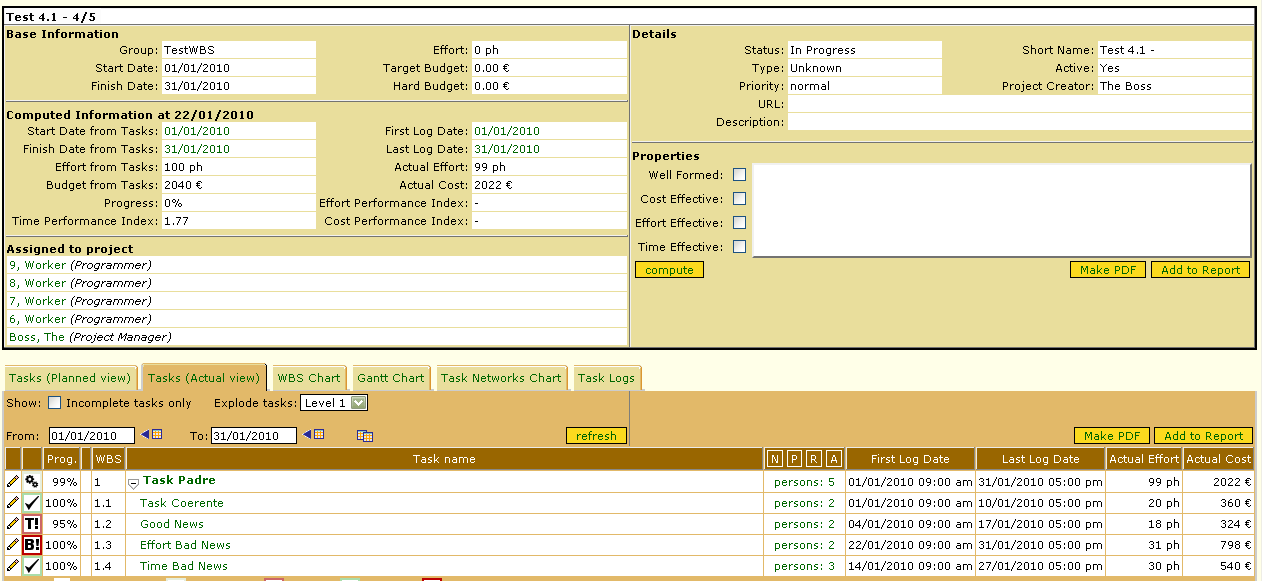
\includegraphics[width=\textwidth]{tests/TEST_WBS/4.1/4.1_4_5/Esempio_1/input_actual.png}
\end{figure}
\newpage

\paragraph{Environment}
\begin{figure}[h!]
\centering
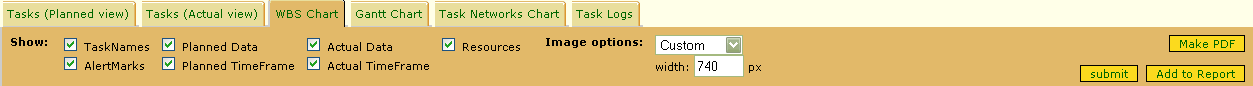
\includegraphics[width=\textwidth]{tests/TEST_WBS/4.1/4.1_4_5/Esempio_1/environment.png}
\end{figure}

\paragraph{Esito}
\begin{figure}[h!]
\centering

\includegraphics[width=\textwidth]{tests/TEST_WBS/4.1/4.1_4_5/Esempio_1/output.png}
\end{figure}
\newpage

\paragraph{Esempio 2}
\paragraph{Input: Planned view, Actual view}
\begin{figure}[h!]
\centering
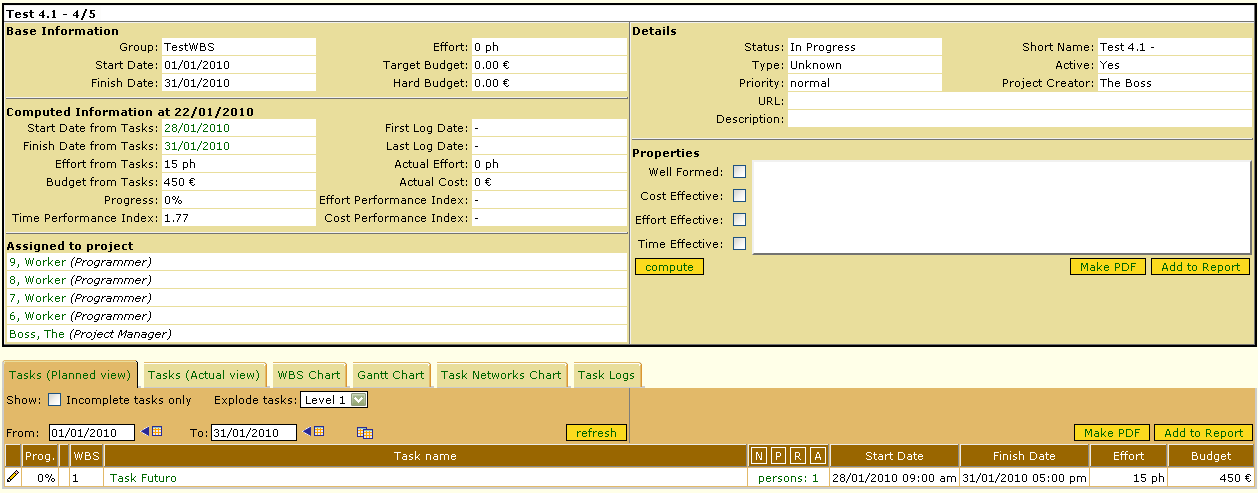
\includegraphics[width=\textwidth]{tests/TEST_WBS/4.1/4.1_4_5/Esempio_2/input.png}
\end{figure}
\begin{figure}[h!]
\centering
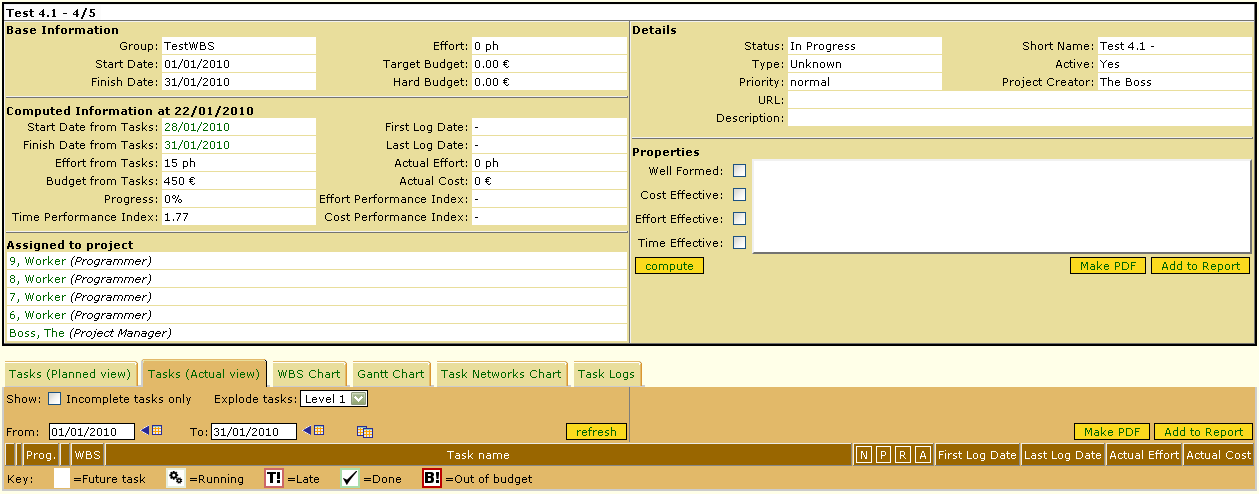
\includegraphics[width=\textwidth]{tests/TEST_WBS/4.1/4.1_4_5/Esempio_2/input_actual.png}
\end{figure}
\newpage

\paragraph{Environment}
\begin{figure}[h!]
\centering
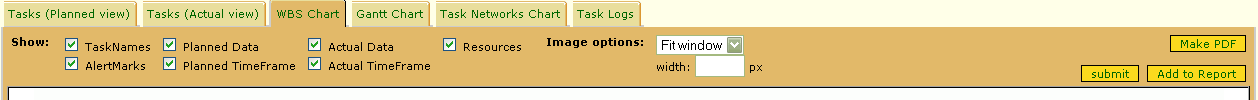
\includegraphics[width=\textwidth]{tests/TEST_WBS/4.1/4.1_4_5/Esempio_2/environment.png}
\end{figure}
\paragraph{Esito}
\begin{figure}[h!]
\centering

\includegraphics[width=\textwidth]{tests/TEST_WBS/4.1/4.1_4_5/Esempio_2/output.png}
\end{figure}
\newpage